\documentclass{article}
\usepackage[margin=0.8in]{geometry}
\usepackage{tikz}
\begin{document}
\section*{Retained p739 plan enrollment audit}
Observations only. This native checker compared retained gate, cohort16 and fresh-session plans. It executed no solver, generated no plan and took no new measurement.\par
Gate workloads:60. Resolved arms:3. Gate executions:1080. Matched executions:1080; missing:0; duplicates:0; seed mismatches:0. Sequence positions differing between gate and cohort subset:900.\par
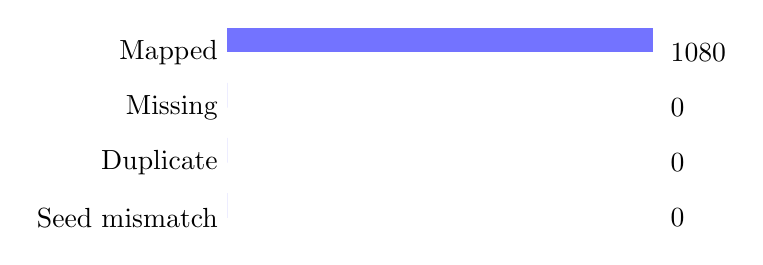
\begin{tikzpicture}[x=0.005cm,y=0.7cm]
\node[anchor=east] at (0,-0) {Mapped};\fill[blue!55] (0,-0) rectangle (1080,--0.45);\node[anchor=west] at (1100,-0) {1080};
\node[anchor=east] at (0,-1) {Missing};\fill[blue!55] (0,-1) rectangle (0,-0.55);\node[anchor=west] at (1100,-1) {0};
\node[anchor=east] at (0,-2) {Duplicate};\fill[blue!55] (0,-2) rectangle (0,-1.55);\node[anchor=west] at (1100,-2) {0};
\node[anchor=east] at (0,-3) {Seed mismatch};\fill[blue!55] (0,-3) rectangle (0,-2.55);\node[anchor=west] at (1100,-3) {0};
\end{tikzpicture}\par
Full workload and resolved arm objects are compared, including original IDs. Algorithm seeds are parsed as exact unsigned64bit integers. Mapping rows retain both sequence positions and both seed values. This verifies membership only; it is not general admission or authority to launch the remaining1200 targets.\par
\subsection*{Input integrity}
Gate: \texttt{\small bc57819e43862f5d9c9aee0f13b983fec186b2dd14dbc8b921d8999acc4b6776}\par
Cohort16: \texttt{\small 35e6311a7105a29c2459543ad0b281ed91e43aa63a99f66226f95a1f3c9cc2ba}\par
Fresh: \texttt{\small bc57819e43862f5d9c9aee0f13b983fec186b2dd14dbc8b921d8999acc4b6776}\par
\par Fresh full plan equality: true. Gate-to-cohort bijection: true.\par
Full machine-readable evidence and all1080 mapping rows are in audit.json; mapping.svg contains the corresponding count graph.
\end{document}
